% !TeX program = xelatex
% UTF-8；使用 XeLaTeX 编译。所有图形均由 TikZ 绘制，无外部图片依赖。
\documentclass[UTF8,zihao=-4]{ctexart}
\usepackage[a3paper,landscape,left=22mm,right=12mm,top=10mm,bottom=10mm]{geometry}
\usepackage{amsmath,amssymb,array,graphicx,xcolor,tikz}
\usetikzlibrary{calc,arrows.meta,shapes.geometric,decorations.pathreplacing}
\pagestyle{empty}
\setlength{\parindent}{0pt}
\setlength{\parskip}{1.4pt}
\setlength{\abovedisplayskip}{2pt}
\setlength{\belowdisplayskip}{2pt}
\setlength{\abovedisplayshortskip}{1pt}
\setlength{\belowdisplayshortskip}{1pt}
\setlength{\jot}{0.5pt}
\renewcommand{\arraystretch}{1.12}
\definecolor{answerred}{RGB}{174,24,28}
\newif\ifanswers
% ANSWER_SWITCH
\newcommand{\red}[1]{{\color{answerred}#1}}
\newcommand{\ans}[1]{\ifanswers\red{#1}\fi}
\newcommand{\blank}[2][3em]{（\makebox[#1][c]{\ans{#2}}）}
\newcommand{\starscore}{\tikz[baseline=-.45ex]{\node[draw,star,star points=5,star point ratio=2.3,minimum size=.9em,inner sep=0pt,line width=.32pt]{};}}
\newcommand{\score}[1]{（#1\starscore）}
\newcommand{\sect}[1]{\par\vspace{2.5pt}{\heiti\zihao{4}#1}\par\vspace{1pt}}
\newcommand{\qn}[1]{\par\noindent #1.\ }
\newcommand{\circled}[1]{\tikz[baseline=(n.base)]{\node[draw,circle,inner sep=0.6pt,minimum size=1.08em,font=\small](n){#1};}}
\newcommand{\cmp}[1]{\tikz[baseline=(n.base)]{\node[draw,circle,inner sep=0pt,minimum size=1.25em](n){\ans{\(#1\)}};}}
\newcommand{\opts}[4]{\par\noindent\begin{tabular*}{\linewidth}{@{}l@{\extracolsep{\fill}}lll@{}}A.\ #1&B.\ #2&C.\ #3&D.\ #4\end{tabular*}\par}
\newsavebox{\areabox}
\newlength{\areaheight}
\newcommand{\ansarea}[2]{%
  \par\begingroup
  \sbox{\areabox}{\begin{minipage}[t]{\linewidth}\vspace{0pt}
    \color{answerred}\fontsize{10.6}{13}\selectfont
    \renewcommand{\arraystretch}{1}\setlength{\jot}{0pt}#2
  \end{minipage}}%
  \setlength{\areaheight}{\dimexpr\ht\areabox+\dp\areabox+4pt\relax}%
  \ifdim\areaheight<#1\setlength{\areaheight}{#1}\fi
  \noindent\begin{minipage}[t][\areaheight][t]{\linewidth}\vspace{0pt}
    \ifanswers\usebox{\areabox}\fi
  \end{minipage}\par\endgroup}
\newcommand{\solmath}[1]{\(\displaystyle\begin{aligned}[t]#1\end{aligned}\)}
\newlength{\oralheight}\newlength{\calcheight}
\ifanswers
  \setlength{\oralheight}{16.2mm}\setlength{\calcheight}{24.7mm}
\else
  \setlength{\oralheight}{6.2mm}\setlength{\calcheight}{39.7mm}
\fi
\newcommand{\calccell}[2]{\begin{minipage}[t][\calcheight][t]{\linewidth}\linespread{1}\fontsize{10.6}{12.6}\selectfont
  \renewcommand{\arraystretch}{1}\setlength{\jot}{0pt}
  \ifanswers
  {\color{answerred}\(\displaystyle\begin{aligned}[t]&\textcolor{black}{#1}#2\end{aligned}\)}
  \else\(\displaystyle #1\)\fi
\end{minipage}}
\newcommand{\oralcell}[3]{\begin{minipage}[t][\oralheight][t]{\linewidth}\linespread{1}\fontsize{10.6}{12.6}\selectfont
  \renewcommand{\arraystretch}{1}\setlength{\jot}{0pt}
  \(#1=\ans{#2}\)
  \ifanswers\par{\color{answerred}\fontsize{9.4}{10.5}\selectfont
  \(\begin{aligned}[t]#3\end{aligned}\)}\fi
\end{minipage}}
\newcommand{\giftgraph}{%
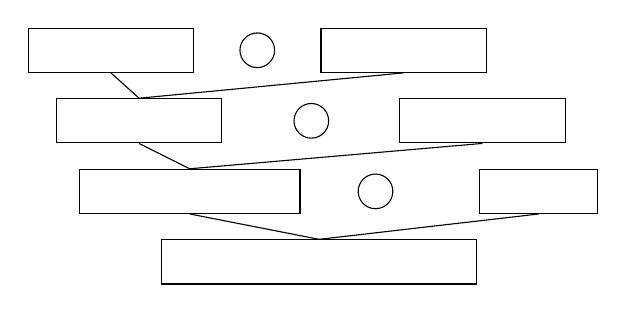
\begin{tikzpicture}[x=14.3mm,y=11.2mm,baseline=(current bounding box.center),
  box/.style={draw,minimum width=21mm,minimum height=5.6mm,inner sep=0pt,font=\small},
  op/.style={draw,circle,minimum size=4.4mm,inner sep=0pt,font=\small}]
\node[box](a) at(0,2.4){\ans{26}};
\node[box](b) at(2.6,2.4){\ans{14}};
\node[op] at(1.3,2.4){\ans{\(+\)}};
\node[box](c) at(.25,1.6){\ans{40}};
\node[box](d) at(3.3,1.6){\ans{3}};
\node[op] at(1.78,1.6){\ans{\(\times\)}};
\node[box,minimum width=28mm](e) at(.7,.8){\ans{120}};
\node[box,minimum width=15mm](f) at(3.8,.8){\ans{18}};
\node[op] at(2.35,.8){\ans{\(+\)}};
\node[box,minimum width=40mm](g) at(1.85,0){\ans{138}};
\draw(a.south)--(c.north) (b.south)--(c.north);
\draw(c.south)--(e.north) (d.south)--(e.north);
\draw(e.south)--(g.north) (f.south)--(g.north);
\end{tikzpicture}}
\newcommand{\smalltriangle}{%
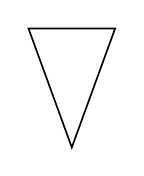
\begin{tikzpicture}[baseline=(current bounding box.center)]
\draw[line width=.6pt](-.55,.65)--(.55,.65)--(0,-.86)--cycle;
\end{tikzpicture}}
\newcommand{\hangingpicture}{%
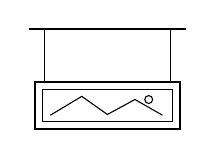
\begin{tikzpicture}[x=5mm,y=5mm,baseline=(current bounding box.center)]
\draw[line width=.7pt](-.2,2.5)--(3.8,2.5);
\draw[line width=.6pt](.2,2.5)--(.2,1.15) (3.4,2.5)--(3.4,1.15);
\draw[line width=.7pt](-.05,-.05)rectangle(3.65,1.15);
\draw[line width=.3pt](.15,.15)rectangle(3.45,.95);
\draw[line width=.4pt](.35,.3)--(1.15,.78)--(1.8,.32)--(2.5,.7)--(3.2,.3);
\draw(2.85,.7)circle(.1);
\end{tikzpicture}}
\newcommand{\stationdrawing}{%
\begin{tikzpicture}[x=10.8mm,y=10.8mm,baseline=(current bounding box.center)]
\draw[line width=.65pt](0,-.1)--(0,3.3)node[above]{$m$};
\draw[densely dotted,line width=.65pt](1.65,-.1)--(1.65,3.3)node[above,font=\small]{等候线};
\foreach \n/\y in {1/2.85,2/1.9,3/.35}{
 \fill(0,\y)circle(1.5pt);
 \node[left=4pt] at(0,\y){\circled{\n}};}
\coordinate(A)at(1.65,.82);\fill(A)circle(1.5pt);\node[right=3pt]at(A){$A$};
\ifanswers
\coordinate(D)at(0,.82);
\draw[answerred,dashed,line width=.8pt](D)--(A);
\draw[answerred,line width=.65pt](0,1.04)--(.22,1.04)--(.22,.82);
\fill[answerred](D)circle(1.9pt);
\node[answerred,left=2pt]at(D){\circled{4}\,$D$};
\fi
\end{tikzpicture}}
\newcommand{\givenlengths}{%
\begin{tikzpicture}[baseline=(current bounding box.center)]
\draw(0,.1)--(0,0)--(3.4,0)--(3.4,.1);
\node[below]at(1.7,0){$a$};
\draw(4.3,.1)--(4.3,0)--(6.85,0)--(6.85,.1);
\node[below]at(5.575,0){$b$};
\end{tikzpicture}}
\newcommand{\construction}{%
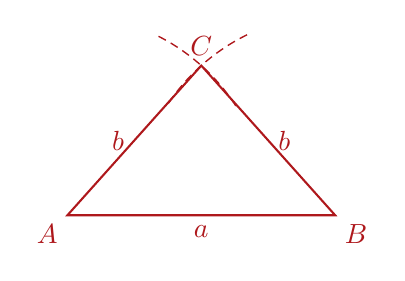
\begin{tikzpicture}[x=8.5mm,y=8.5mm,baseline=(current bounding box.center)]
\coordinate(A)at(0,0);\coordinate(B)at(4,0);\coordinate(C)at(2,{sqrt(5)});
\draw[answerred,densely dashed,line width=.5pt](A)++(33:3)arc(33:64:3);
\draw[answerred,densely dashed,line width=.5pt](B)++(116:3)arc(116:147:3);
\draw[answerred,line width=.75pt](A)--node[below]{$a$}(B)--node[right]{$b$}(C)--node[left]{$b$}cycle;
\foreach \p/\pos in {A/below left,B/below right,C/above}
 \node[\pos,answerred]at(\p){$\p$};
\end{tikzpicture}}
\newcommand{\receipt}{%
\begingroup\small\setlength{\tabcolsep}{4pt}
\begin{tabular}{|c|c|c|c|c|}\hline
\multicolumn{5}{|c|}{购物小票}\\\hline
编号&商品&单位&数量&单价\\\hline
1&\shortstack{笔记本}&个&45&
\tikz[baseline=-.6ex]{\node[draw,star,star points=10,star point ratio=1.65,minimum width=10mm,minimum height=6mm,inner sep=0pt,font=\small]{\ifanswers\red{3元}\else\phantom{3元}\fi};}\\\hline
2&碳素笔&支&80&2元\\\hline
\multicolumn{5}{|l|}{总计金额：295元}\\\hline
\end{tabular}\endgroup}
\newcommand{\tigerprices}{%
\begingroup\small\setlength{\tabcolsep}{7pt}
\begin{tabular}{|c|c|c|}\hline
种类&黄河虎&团圆虎\\\hline
售价&每只62元&每只58元\\\hline
\end{tabular}\endgroup}
\newcommand{\tunneldiagram}{%
\begin{tikzpicture}[x=1mm,y=1mm,>=Stealth,font=\small]
\draw[answerred,line width=.6pt](0,0)rectangle(147,6);
\draw[answerred](78.7,0)--(78.7,6) (90,0)--(90,6);
\draw[answerred,->](2,10)--(76,10);
\draw[answerred,->](145,10)--(93,10);
\node[answerred,above]at(39,12){甲队12天};
\node[answerred,above]at(119,12){乙队12天};
\node[answerred]at(39,3){$29\times12=348$米};
\node[answerred]at(119,3){$21\times12=252$米};
\node[answerred,font=\fontsize{8.2}{9}\selectfont]at(84.35,3){50米};
\node[answerred,font=\small,above]at(84.35,6){剩余};
\draw[answerred](0,-4)--(147,-4) (0,-5.5)--(0,-2.5) (147,-5.5)--(147,-2.5);
\node[answerred,below]at(73.5,-4){全长？米};
\end{tikzpicture}}
\newlength{\colwidth}
\setlength{\colwidth}{\dimexpr(\textwidth-10mm)/2\relax}
\newsavebox{\leftpanel}\newsavebox{\rightpanel}
\newenvironment{panel}{\begin{minipage}[t]{\colwidth}\vspace{0pt}\fontsize{11.4}{15}\selectfont}{\end{minipage}}
\newcommand{\shipspread}[1]{%
\typeout{PANEL-#1-LEFT=\the\dimexpr\ht\leftpanel+\dp\leftpanel\relax}
\typeout{PANEL-#1-RIGHT=\the\dimexpr\ht\rightpanel+\dp\rightpanel\relax}
\noindent\usebox{\leftpanel}\hfill\usebox{\rightpanel}
\begin{tikzpicture}[remember picture,overlay]
\draw[line width=.5pt]($(current page.north west)+(20mm,-10mm)$)--($(current page.north east)+(-10mm,-10mm)$);
\draw[line width=.35pt]($(current page.north west)+(215mm,-10mm)$)--($(current page.south west)+(215mm,12mm)$);
\ifnum#1=1
\draw[dashed,line width=.45pt]($(current page.north west)+(19mm,-10mm)$)--($(current page.south west)+(19mm,12mm)$);
\node[rotate=90,font=\heiti\small]at($(current page.west)+(15mm,0)$){密\hspace{40mm}封\hspace{40mm}线};
\node[rotate=90,font=\heiti\small]at($(current page.west)+(8mm,58mm)$){\underline{\hspace{16mm}}年级\underline{\hspace{12mm}}班\quad 姓名：\underline{\hspace{25mm}}};
\node[rotate=90,font=\heiti\small]at($(current page.west)+(8mm,-76mm)$){小学数学四年级阶段测试试题};
\fi
\node[font=\small]at($(current page.south)+(0,6mm)$){第#1页\quad 共2页\ifanswers\quad 答案版\fi};
\end{tikzpicture}}
\begin{document}
% 第一张：保持原卷的左右栏顺序。
\begin{lrbox}{\leftpanel}\begin{panel}
\fontsize{13}{18.9}\selectfont\setlength{\parskip}{2pt}
\begin{center}
{\heiti\fontsize{14}{19}\selectfont 2026——2027学年度第一学期阶段测试}\\[2pt]
{\heiti\fontsize{17}{21}\selectfont 四年级数学试题}\quad{\small（试题99\starscore\quad 卷面1\starscore）}
\end{center}\vspace{-3pt}
\sect{一、填空题。\score{26}}
\qn{1}根据运算顺序，把$71-47=24$，$24\times3=72$，$576\div72=8$，改写成综合算式是
\blank[20em]{$576\div[(71-47)\times3]$}。
\par\noindent\begin{minipage}[t]{.52\linewidth}\vspace{0pt}
\qn{2}一支钢笔26元，一个笔记本14元，一套文具礼盒的价格比钢笔和笔记本单价和的3倍多18元。一套文具礼盒\blank{138}元。根据题意进行分析，将右图填写完整。
\end{minipage}\hfill
\begin{minipage}[t]{.46\linewidth}\vspace{1pt}\centering\giftgraph\end{minipage}
\qn{3}屋顶钢架是利用了\blank{三角}形的稳定性。
\par\noindent\begin{minipage}[c]{.89\linewidth}
\qn{4}右图所示，按角分类属于\blank{锐角}三角形，按边分类属于\blank{等腰}三角形，它的一个底角是$70^\circ$，另外两个内角分别是\blank[2em]{70}$^\circ$和\blank[2em]{40}$^\circ$。
\end{minipage}\hfill\begin{minipage}[c]{.08\linewidth}\smalltriangle\end{minipage}
\qn{5}马小虎不小心把$30\times(\square+6)$错算成$30\times\square+6$。计算结果与正确结果相差\blank{174}。
\qn{6}王爷爷用一根长90厘米的竹条做风筝，风筝是一个腰长为29厘米的等腰三角形，这个风筝的底边长\blank{32}厘米。
\qn{7}今年的秋假小明一家打算去北京游玩，如果请你帮忙制作一份家庭旅游计划，这份家庭旅游计划包括\blank[4.6em]{旅游时间}、\blank[4.6em]{旅游路线}、\blank[4.6em]{费用预算}等
\qn{8}在$\bigcirc$里填上“$>$”、“$<$”或“$=$”
\par\noindent\hspace{1em}$12\times99$\cmp{<}$12\times100-1$\hfill
$600-123+377$\cmp{>}$600-(123+377)$\hspace{1em}
\qn{9}把一张正方形纸对折两次后，折痕可能互相\blank{垂直}，也可能互相\blank{平行}。
\sect{二、选择题。\score{7}}
\qn{1}计算器的数字键3坏了，计算$27\times36$时，下面的计算方法中，不能得出正确结果的是\blank{B}
\opts{$27\times4\times9$}{$27\times40-4$}{$27\times6\times6$}{$27\times18\times2$}
\qn{2}一个等腰三角形的两条边分别是3厘米和8厘米，那么它的周长是\blank{B}。
\opts{14CM}{19CM}{14CM或19CM}{无法确定}
\qn{3}通过直线外一点可以画\blank[2em]{A}条直线与已知直线互相垂直，\blank[2em]{A}条直线与已知直线平行。
\opts{1}{2}{3}{无数}
\qn{4}下面说法正确的有\blank{B}个
\ifanswers
\par\vspace{2pt}{\fontsize{9.5}{11.5}\selectfont\color{answerred}
填空第7题答案不唯一，合理即可。选择第3题两空均选A，即各1条。\\
选择第4题只有\circled{1}\circled{2}正确，共2个，选B。\circled{4}中仅面积相等，不能保证拼成平行四边形；应表述为“两个完全一样的三角形”。\par}
\fi
\end{panel}\end{lrbox}
\begin{lrbox}{\rightpanel}\begin{panel}
\fontsize{12}{15}\selectfont
\circled{1}两条直线相交成4个角，如果有一个角是直角，那么其他3个角一定也是直角。\par
\circled{2}正三角形一定是锐角三角形。\par
\circled{3}用三根3厘米、1厘米、2厘米的小棒可以围成一个三角形。\par
\circled{4}用两个大小一样的三角形可以拼成一个平行四边形。
\opts{1}{2}{3}{4}
\qn{5}一个三角形中，有一个角是89度，这个三角形是\blank{D}三角形。
\opts{锐角}{直角}{钝角}{无法确定}
\par\noindent\begin{minipage}[t]{.84\linewidth}\vspace{0pt}
\qn{6}李阿姨把一幅画挂歪了，于是她将挂画的两根绳子的长度调成一样长后，画就正了，这是运用了\blank{C}的道理。
\end{minipage}\hfill\begin{minipage}[t]{.14\linewidth}\vspace{0pt}\centering\hangingpicture\end{minipage}
\par\noindent\begin{tabular*}{\linewidth}{@{}l@{\extracolsep{\fill}}l@{}}
A.\ 两点之间线段最短&B.\ 垂直线段最短\\
C.\ 两条平行线的距离处处相等&D.\ 两条直线间的线段相等。
\end{tabular*}
\sect{三、计算题。}
\qn{1}直接写出得数。\score{10}
\par\noindent\begin{tabular}{@{}p{.245\linewidth}@{}p{.245\linewidth}@{}p{.245\linewidth}@{}p{.265\linewidth}@{}}
\oralcell{24\times5}{120}{}&
\oralcell{12\times15}{180}{}&
\oralcell{360\div8\div5}{9}{={}&45\div5\\={}&9}&
\oralcell{25\times4\div25\times4}{16}{={}&100\div25\times4\\={}&4\times4\\={}&16}\\
\oralcell{26+58}{84}{}&
\oralcell{81-37}{44}{}&
\oralcell{130-30\div6}{125}{={}&130-5\\={}&125}&
\oralcell{630\div42}{15}{}\\
\oralcell{540\div45\div2}{6}{={}&12\div2\\={}&6}&
\oralcell{125\times8}{1000}{}&
\oralcell{25\times3\times4}{300}{={}&25\times4\times3\\={}&100\times3\\={}&300}&
\oralcell{136-45-55}{36}{={}&136-(45+55)\\={}&136-100\\={}&36}
\end{tabular}
\qn{2}怎样简便就怎样算。\score{18}
\par\noindent\begin{tabular}{@{}p{.335\linewidth}@{}p{.31\linewidth}@{}p{.355\linewidth}@{}}
\calccell{627-118+173-82}{\\={}&(627+173)-(118+82)\\={}&800-200\\={}&600}&
\calccell{25\times32\times125}{\\={}&25\times4\times8\times125\\={}&(25\times4)\times(8\times125)\\={}&100\times1000\\={}&100000}&
\calccell{[288\div(295-289)]\times45}{\\={}&[288\div6]\times45\\={}&48\times45\\={}&2160}\\
\calccell{65\times[(384+576)\div12]}{\\={}&65\times[960\div12]\\={}&65\times80\\={}&5200}&
\calccell{37\times99+37}{\\={}&37\times99+37\times1\\={}&37\times(99+1)\\={}&37\times100\\={}&3700}&
\calccell{215-98}{\\={}&215-100+2\\={}&115+2\\={}&117}
\end{tabular}
\sect{四、请按照要求进行作图。\score{4}}
\par\noindent\begin{minipage}[t]{.70\linewidth}\vspace{0pt}
\qn{1}学校进行流感疫苗注射，如图所示，在一条直线$m$上有\circled{1}\circled{2}\circled{3}三个注射台，小方站在$A$点处。如果在直线$m$上再加一个注射台\circled{4}，你认为设在什么位置能距离小方最近？请你画出来
\ifanswers\par\vspace{1pt}\red{\fontsize{10}{12}\selectfont
过点$A$作直线$m$的垂线，垂足$D$处设注射台\circled{4}。线段$AD$最短。\par}\fi
\end{minipage}\hfill\begin{minipage}[t]{.27\linewidth}\vspace{0pt}\centering\stationdrawing\end{minipage}
\end{panel}\end{lrbox}
\shipspread{1}
\newpage
% 第二张：作图第2题和应用题仍在原来的栏位。
\begin{lrbox}{\leftpanel}\begin{panel}
\qn{2}用直尺和圆规画一个以$a$为底，以$b$为腰的等腰三角形。（保留作图痕迹。）
\par\noindent\begin{minipage}[t][31mm][t]{.55\linewidth}\vspace{5pt}\givenlengths
\ifanswers\par\vspace{6pt}\red{\small
作线段$AB=a$。分别以$A$、$B$为圆心，以$b$为半径画弧，两弧交于$C$，连接线段$AC$、$BC$。\\[2pt]
$AB=a$，$AC=BC=b$，保留两段圆弧。}\fi
\end{minipage}\hfill\begin{minipage}[t][31mm][t]{.41\linewidth}\vspace{4pt}\ifanswers\centering\construction\fi\end{minipage}
\sect{五、应用题。\score{34}}
\par\noindent\begin{minipage}[t]{.61\linewidth}\vspace{0pt}
\qn{1}为了增强同学们的身体素质，学校每周都要进行体能测试，学校为每个优胜者发奖品。45个笔记本和80支碳素笔，电子小票如右图。请你算算每个笔记本的单价是多少元？\score{5}
\end{minipage}\hfill\begin{minipage}[t]{.37\linewidth}\vspace{2pt}\centering\receipt\end{minipage}
\ansarea{27mm}{\solmath{&(295-2\times80)\div45\\={}&(295-160)\div45\\={}&135\div45\\={}&3\text{（元）}}\par
答：每个笔记本的单价是3元。}
\qn{2}一本影集有16页，明明趁十一长假出去游玩，照了184张照片，如果影集正面和反面各放6张照片，这本影集够用吗？\score{5}
\ansarea{20mm}{%
\begin{minipage}[t]{.30\linewidth}\vspace{0pt}
\solmath{&6\times2\times16\\={}&12\times16\\={}&192\text{（张）}}
\end{minipage}\hfill
\begin{minipage}[t]{.66\linewidth}\vspace{0pt}
$192>184$，$192-184=8$（张）。\\
答：这本影集够用，还可以放8张照片。\end{minipage}}
\qn{3}中医药方“清肺排毒汤”用量最多的药材如下。\score{5}
\par 石膏：57克\qquad 藿香：比石膏少19克
\par 柴胡：是藿香的3倍。
\par 柴胡的质量是石膏的几倍？
\ansarea{29mm}{\solmath{&(57-19)\times3\div57\\={}&38\times3\div57\\={}&114\div57\\={}&2}\par
答：柴胡的质量是石膏的2倍。}
\qn{4}某公司制作了一批颜色各异的布老虎，其中黄河虎制作了14箱，共980只，团圆虎制作了16箱，共720只。
\par（1）平均每箱黄河虎比每箱团圆虎多多少只？\score{4}
\ansarea{26mm}{\solmath{&980\div14-720\div16\\={}&70-45\\={}&25\text{（只）}}\par
答：平均每箱黄河虎比每箱团圆虎多25只。}
\end{panel}\end{lrbox}
\begin{lrbox}{\rightpanel}\begin{panel}
（2）如表，若黄河虎和团圆虎全部卖出，一共收入多少元？\score{4}
\par\hfill\tigerprices
\ansarea{24mm}{\solmath{&62\times980+58\times720\\={}&60760+41760\\={}&102520\text{（元）}}\par
答：一共收入102520元。}
\qn{5}甲乙两个实力相当的工程队分别从两端同时开凿一条隧道，甲队每天开凿29米，乙队每天开凿21米，12天后还剩50米隧道贯通。这条隧道有多长？（先画图分析数量关系，再解答）\score{6}
\ansarea{26mm}{\centering\tunneldiagram}
\ansarea{29mm}{\solmath{&(29+21)\times12+50\\={}&50\times12+50\\={}&600+50\\={}&650\text{（米）}}\par
答：这条隧道长650米。}
\qn{6}某快递站平均每天需派送快递960件，现有4名快递员，每天可派送快递320件，照这样计算，再招聘几名快递员才能完成任务？\score{5}
\ansarea{46mm}{%
\begin{minipage}[t]{.40\linewidth}\vspace{0pt}
\solmath{&960\div(320\div4)-4\\={}&960\div80-4\\={}&12-4\\={}&8\text{（名）}}
\end{minipage}\hfill
\begin{minipage}[t]{.56\linewidth}\vspace{0pt}
4人每天合计派送320件，每人每天派送$320\div4=80$（件）。\\[2pt]
答：再招聘8名快递员才能完成任务。
\end{minipage}}
\sect{六、附加题：{\normalsize（1题4\starscore，2和3题3\starscore）}}
\qn{1}根据规律写算式。
\par\hspace{1em}$55\times81=4455$，
\par\hspace{1em}$555\times801=444555$，
\par\hspace{1em}$5555\times8001=44445555$，
\par\hspace{1em}\blank[5em]{55555}$\times$\blank[5em]{80001}$=$\blank[8em]{4444455555}
\qn{2}请你快速算出$100-98+96-94+92-\cdots-6+4-2=$\blank{50}。
\qn{3}一个等腰三角形，它一个底角的度数是顶角的4倍。它的顶角是\blank{20}度
\ansarea{22mm}{%
\begin{minipage}[t]{.56\linewidth}\vspace{0pt}
第2题：\par
\solmath{&100-98+96-94+\cdots+4-2\\={}&(100-98)+(96-94)+\cdots+(4-2)\\={}&2\times25\\={}&50}
\end{minipage}\hfill
\begin{minipage}[t]{.41\linewidth}\vspace{0pt}
第3题：\par
\solmath{&180^\circ\div(4+4+1)\\={}&180^\circ\div9\\={}&20^\circ}\par
顶角1份，两个底角各4份，共9份。
\end{minipage}}
\end{panel}\end{lrbox}
\shipspread{2}
\end{document}
